\section{Introduction}
\label{sec:Introduction}

With widespread use of social media, such as blogging services or social
network services (SNS), today we can publish information
on the Web more easily than before.  Recently,
microblogging services have especially been growing rapidly.

Microblogs are a new type of services which have both characteristics
of blogs and SNS.  In microblogs, users can post short messages more
easily and quickly than in conventional blogs or SNS.
Microblogs are not necessarily regarded as media for
publishing useful information to the public, and many microblog users
post messages more casually than in conventional blogs or
SNS.  Because of these characteristics of microblogs, a
large number of messages are posted every
day, and the messages contain various types of contents, from personal
notes or life logs to useful information or discussion on specific
topics.

Among many microblogs,
Twitter\footnote{\url{http://twitter.com/}} is especially growing
explosively.  As of 2013 Octover, Twitter has over 218 million monthly
active users in the world, and more than 500 million
messages are posted on it per day\cite{TweetsData}.  In Twitter, users
can post short messages with at most 140 characters, which are called
tweets.
The most distinctive feature of Twitter is its mechanism of
\emph{''follow''}.  In Twitter, if a user follows other users, all
tweets by these followee users are retrieved in real time, and are
shown in a list sorted in the reverse chronological order, as shown in
Figure~\ref{fig:twitter}.  This list is called the \emph{''timeline''}
of the follower users.  The mechanism of follow is more casual than
user-linking functions in ordinary SNS; it does not basically require the
permission by the followee, and does not necessarily imply reciprocal
relationship. Another important function in Twitter is the
\emph{''reply''} function, by which a user can post a message as a
reply to another user.  By using this function, users can use Twitter
for conversation, as in instant messaging services.

\begin{figure}[t]
\begin{center}
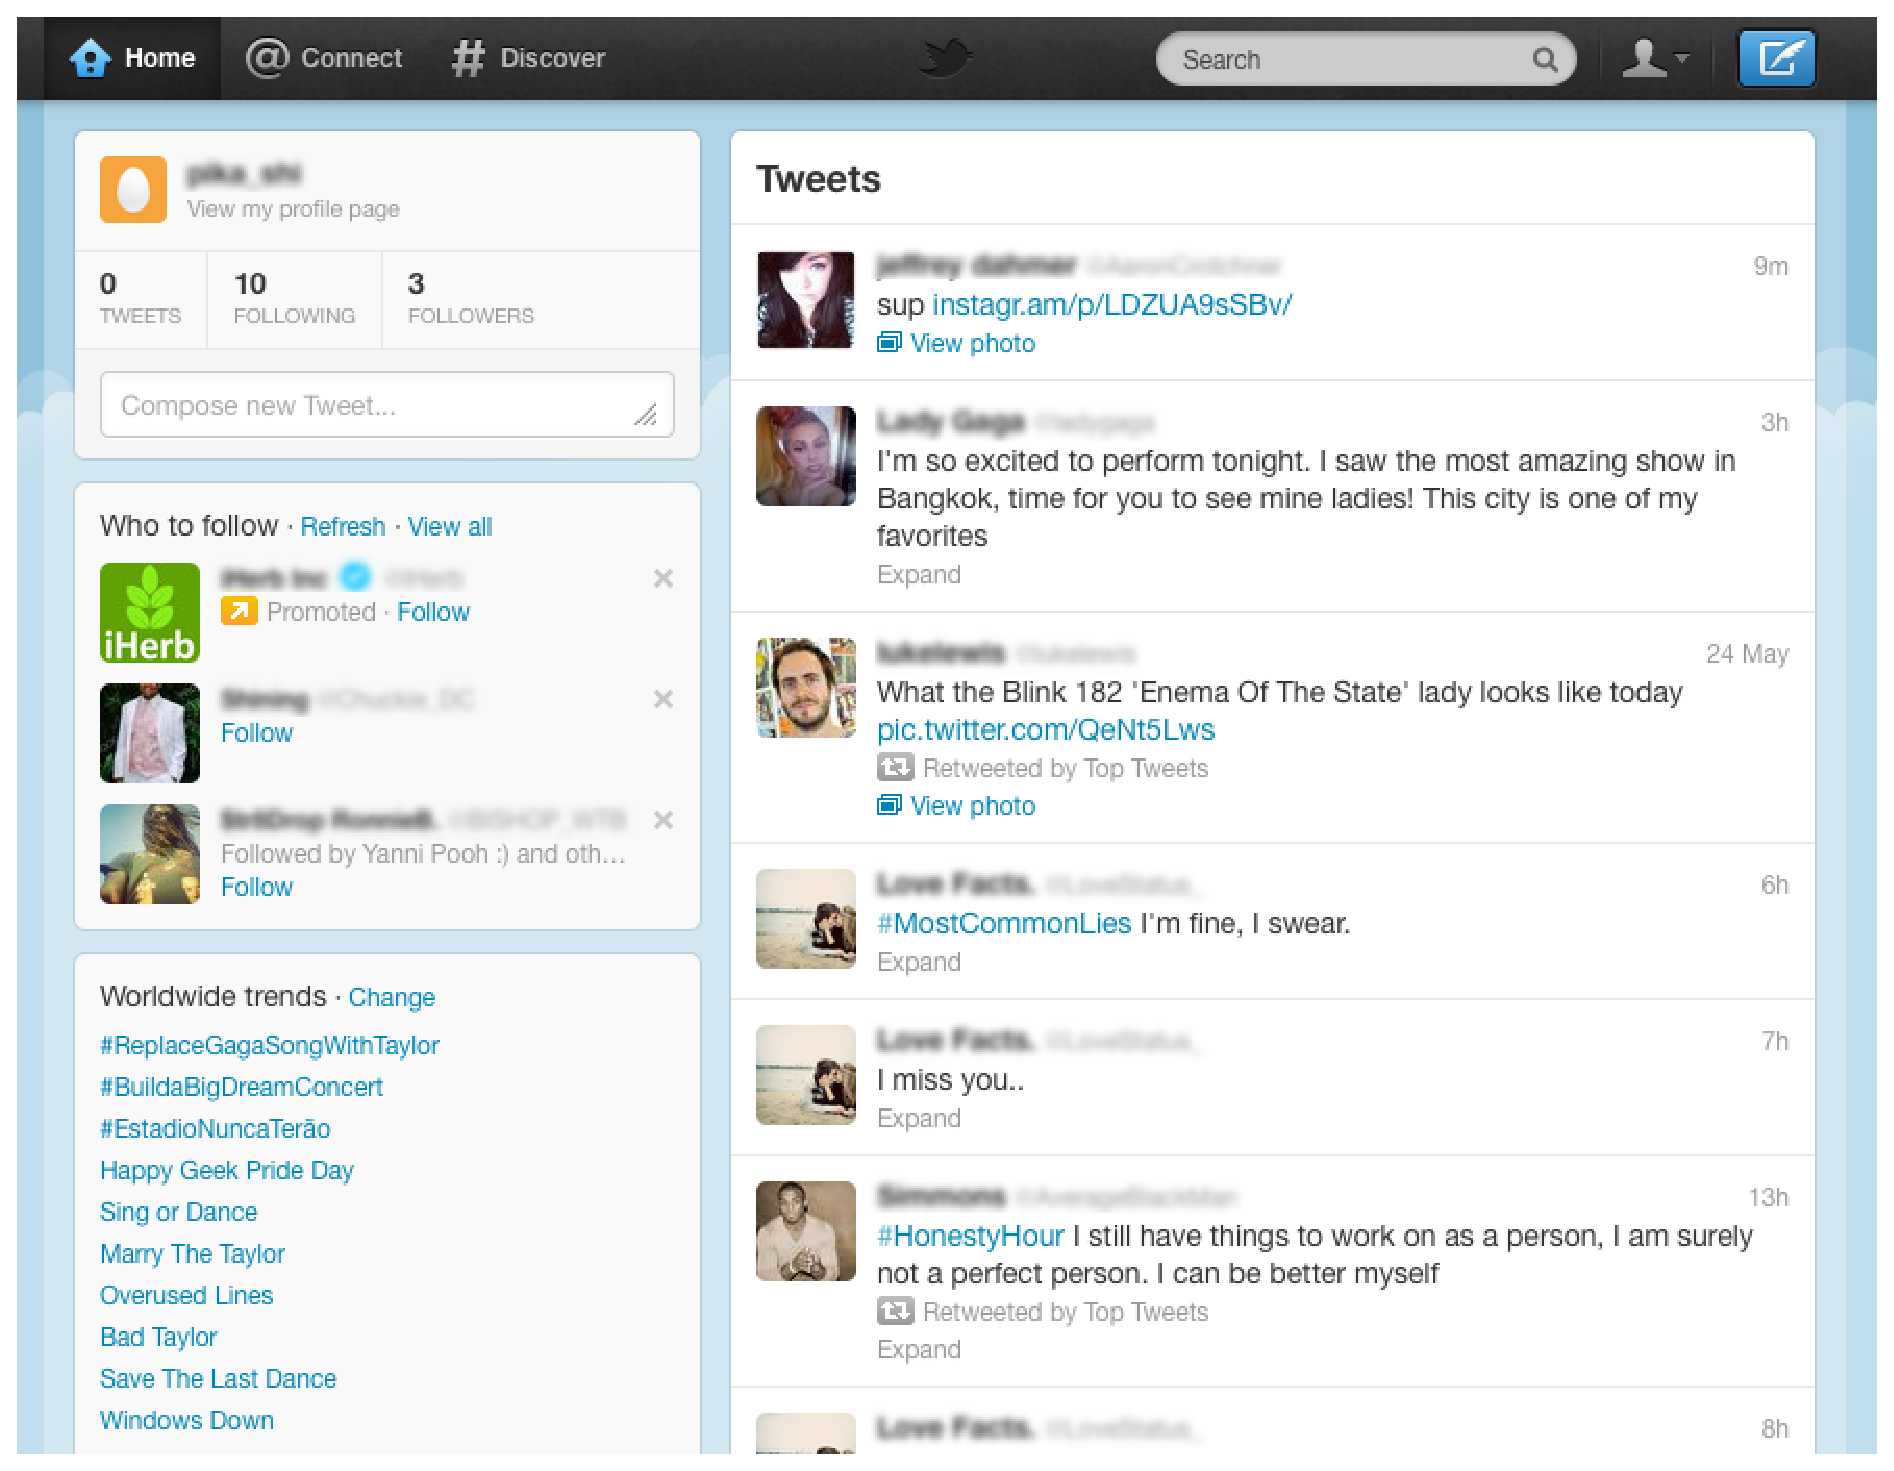
\includegraphics[width=14cm]{images/screen_shot.eps}
 \caption{An example of a user's timeline in Twitter}
\label{fig:twitter}
\end{center}
\end{figure}

As Twitter has characteristics similar to various conventional social
media, so it is used for many purposes.  Some users, e.g., Twitter
accounts owned by major news companies, publish general information on
various topics to the wide public, while some users publish
information specific to certain topics.  There are also users that use
Twitter for the communication with their friends or others.  Because
of this characteristic of Twitter, it has attracted great attention as
a new type of social media.

As explained above, Twitter is used for various purposes.  As a result,
the breadth of target scope of information publishing varies greatly
from users to users.
%tajima:情報発信の対象範囲が様々だというのは説明したとして,次に,その
%場合になぜ対象範囲に基づいてユーザを分類をすることが重要なのか,なぜそ
%ういうことを研究するのに必然性があるのかということについて,ここにもっ
%と書けませんか.
In this study, we propose a method to classify
Twitter users based on how broad the target scope of
their information publishing is, i.e., whether they publish information
to the wide public or publish information to specific groups of users.
In the former case, we say \emph{``target specificity is
low''}, and in the latter case, we say \emph{``target specificity
is high''}.

In our classification method, we use the information on the
consistency among the followers of each user.  If most of the
followers of a user have some noticeable characteristics in common, we
determine that the user publishes information only to users that have
some specific interests or characteristics.  On the other hand, if the
followers of the user have no common noticeable characteristics, it
means that the user is followed by a wide variety of users, and we
determine that the user publishes information to the wide public.

In this study, we also focus on the causes of such target specificity.
We propose a method of determining why target scope of a given user,
which has been classified as a user with high target specifity, is
restricted to some specific type of users.  A large portion of Twitter
users have high target specificity, and the causes of their target
specificity vary from users to users.  For example, some users use
Twitter for the communication with the friends, or for announcing some
information to members of a certain organization.  Messages by such a
user may include various topics and may not be restricted to some
specific topic, but they intend to publish information only to
specific users.  Therefore, their target specificity is high.  On the
other hand, a user who publishes technical information about computer
programming does not have specific users in his mind, but their
messages include only specific topics, i.e., programming, and they
publish information only to users who are interested in programming.
Such a user also have high target specificity.

We roughly classify the causes of target specificity into two types:
(1) topic specificity, i.e., target specificity of a user is high
because the user publishes information on some specific topics, and
(2) user specificity, i.e, target specificity of a user is high
because the user publishes information to a specific group of users.
A ``specific group of users'' means a set of users which can be
defined extensionally, such as friends of some users or members of
some organization.  A set of users which can be defined only
intensionally, e.g., a set of users that are interested in
programming, is not regarded as a ``specific group'' here.

We classify users based on the causes of their high target specificity
by constructing a classifier which determines whether a
user belongs only to category (1), only to category (2), or belong to
both category (1) and (2).  Our classifier uses various features of
users which correlate with each category.  Figure~\ref{fig:Flow} shows
main components of our method and information flow among them.

\begin{figure}[t]
\begin{center}
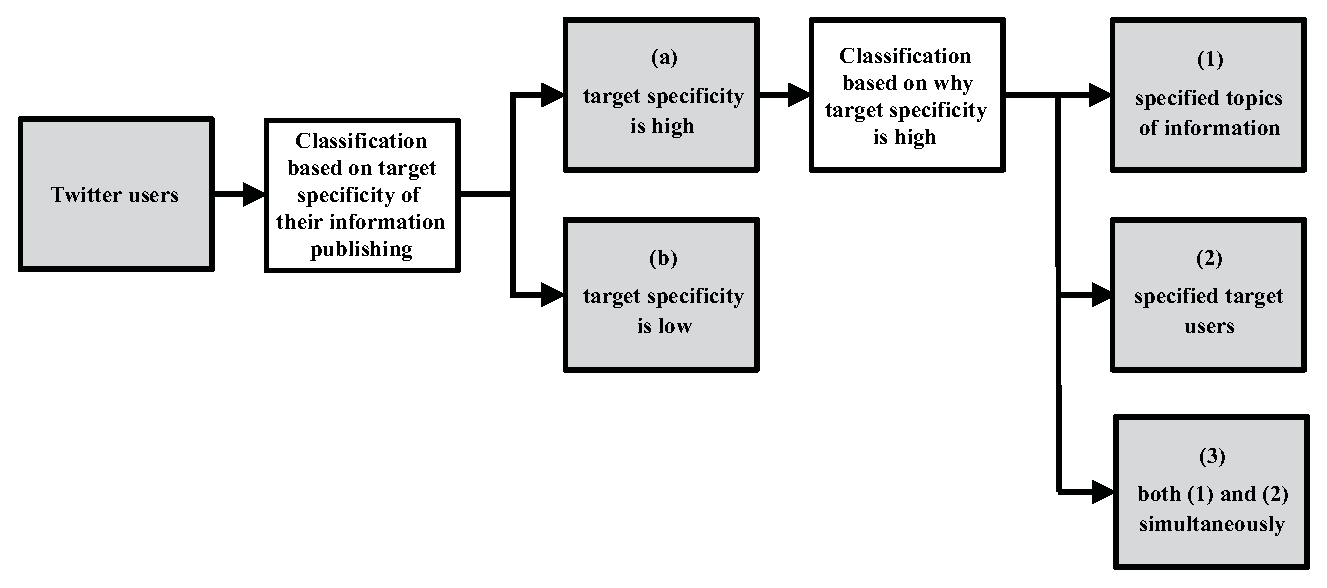
\includegraphics[width=14cm]{images/flow.eps}
 \caption{Main components of our method and information flow among them}
\label{fig:Flow}
\end{center}
\end{figure}

On the Web, it is hard to know what kinds of users each Web page
targets to.  In Twitter, however, we can guess what kinds of users
each user targets to by examining the followers of the user.  By using
this information, we can determine whether a given user has high
target specificity or not.

Twitter user classification by our method can be utilized in Twitter
search systems.  In current Twitter search systems, we input query
keywords and receive messages including the keywords.  In these
systems, however, a search result includes messages with various
target scope.  As a result, it frequently happens that messages
relevant to the querying user are buried in many messages whose target
scope do not include the querying user.  For example, when a user
submits a query ``MacBook Air'' to the Twitter search system, what
kinds of messages he needs depends on the situation.  The user may
need public news about MacBook Air, may need technical information
about MacBook Air, or may need ordinary users' reviews of MacBook Air
in order to decide to or not to buy a MacBook Air.  In the current
Twitter search systems, however, these different types of messages are
mixed in a search result.  In such a case, we can use our Twitter user
classification method in order to classify messages in the search
result, so that messages that the user wants are not buried in many
other types of messages.

The contribution of this paper is summarized as follows.

\begin{itemize}
\item We propose a new classification scheme of Twitter users which is
based on target specificity their information publishing.
\item We show a method of classifying Twitter users in the scheme above.
\item We also show a method of determining the causes of high target
specificity for users that are classified as users with high target specificity.
\end{itemize}

The rest of this paper is organized as follows.  Next chapter explains
some related work and clarify the relationship between our study and
the related work.
We then define target specificity of information publishing and
formulate our problem in \ref{sec:Target Specificity}. In
\ref{sec:Target Specificity}, we also discuss why target scope of some
user is restricted to some specific type of users.  In
\ref{sec:ClassificationMethod1}, we explain the method of classifying
Twitter users based on their target specificity of information
publishing.  In addition, we explain the method of determining the
causes of target specificity of the users classified as high target
specificity users in \ref{sec:ClassificationMethod2}.  Then in \ref{sec:Experiment},
we show the results obtained from experiments we conducted to
evaluate our methods.  \ref{sec:Conclusion} concludes the paper.
